%%%%%%%%%%%%%%%%%%%%%%%%%%%%%%%%%%%%%%%%%%%%%%%
%%% Template for lab reports used at STIMA
%%%%%%%%%%%%%%%%%%%%%%%%%%%%%%%%%%%%%%%%%%%%%%%

%%%%%%%%%%%%%%%%%%%%%%%%%%%%%% Sets the document class for the document
% Openany is added to remove the book style of starting every new chapter on an odd page (not needed for reports)
\documentclass[10pt,english, openany]{book}

%%%%%%%%%%%%%%%%%%%%%%%%%%%%%% Loading packages that alter the style
\usepackage[]{graphicx}
\usepackage[]{color}
\usepackage{alltt}
\usepackage[T1]{fontenc}
\usepackage[utf8]{inputenc}
\setcounter{secnumdepth}{3}
\setcounter{tocdepth}{3}
\setlength{\parskip}{\smallskipamount}
\setlength{\parindent}{0pt}
\usepackage{multicol}

% Set page margins
\usepackage[top=100pt,bottom=100pt,left=68pt,right=66pt]{geometry}

% Package used for placeholder text
\usepackage{lipsum}

% Prevents LaTeX from filling out a page to the bottom
\raggedbottom

% Adding both languages
\usepackage[english, italian]{babel}

% All page numbers positioned at the bottom of the page
\usepackage{fancyhdr}
\fancyhf{} % clear all header and footers
\fancyfoot[C]{\thepage}
\renewcommand{\headrulewidth}{0pt} % remove the header rule
\pagestyle{fancy}

% Changes the style of chapter headings
\usepackage{titlesec}
\titleformat{\chapter}
   {\normalfont\LARGE\bfseries}{\thechapter.}{1em}{}
% Change distance between chapter header and text
\titlespacing{\chapter}{0pt}{50pt}{2\baselineskip}

% Adds table captions above the table per default
\usepackage{float}
\floatstyle{plaintop}
\restylefloat{table}

% Adds space between caption and table
\usepackage[tableposition=top]{caption}

% Adds hyperlinks to references and ToC
\usepackage{hyperref}
\hypersetup{hidelinks,linkcolor = black} % Changes the link color to black and hides the hideous red border that usually is created

% If multiple images are to be added, a folder (path) with all the images can be added here 
\graphicspath{ {Figures/} }

% Separates the first part of the report/thesis in Roman numerals
\frontmatter


%%%%%%%%%%%%%%%%%%%%%%%%%%%%%% Starts the document
\begin{document}

%%% Selects the language to be used for the first couple of pages
\selectlanguage{english}


\mainmatter


\begin{centering}

	{\LARGE \textbf{Gebze Technical University}} \\
	{\LARGE \textbf{Computer Engineering}} \\
	    \vspace{2.0cm}
	    
\begin{figure}[htp]
    \centering
    
\includegraphics[width=5cm]{gtu_logo.png}
    
\end{figure}	    
	    
	    \vspace{2.0cm}
	    
	{\LARGE \textbf{System Programming}} \\
	{\LARGE \textbf{CSE344 – 2021}} \\
	    \vspace{3.0cm}
	
	{\LARGE \textbf{MIDTERM-REPORT}} \\
		\vspace{3.0cm}

	{\LARGE \textbf{Yusuf Abdullah ARSLANALP}} \\
	{\LARGE \textbf{151044046}} \\
	    %\vspace{3.0cm}


\end{centering}



\newpage


\section{How I Solved This Problem}
There are three types of thread. These are main thread, H thread and student-for-hire thread. Main thread creates all necessary semaphores and initialize them. After termination of all other threads main thread destroys all created semaphores.

Students for hire are read from the file and filled in to a struct array. The structure of struct as follows:

\begin{figure}[htp]
    \centering
    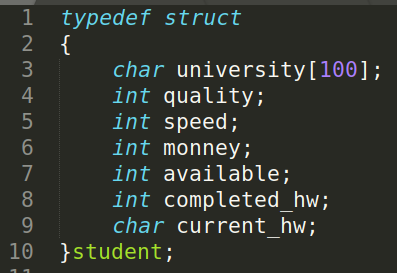
\includegraphics[width=5cm]{struct.PNG}
    
\end{figure}	 

Semaphores are kept as global. So they can be use from every threads. There are used four semaphore and one semaphore array in the homework. Semaphore names in program as follows:

\begin{figure}[htp]
    \centering
    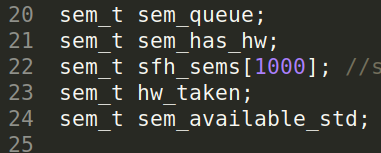
\includegraphics[width=5cm]{sems.PNG}
    
\end{figure}

Every student-for-hire thread has its own semaphore. Inıtially all student-for-hire threads waits with their own semaphores. When main thread decides to assign a homework to one of the student-for-hire it increment semaphore value of the selected student-for-hire. Selected student does the homework. And waits for another assignment.

\section{Which requirements I achieved}

\begin{itemize}
  \item When CTRL-C pressed program terminated gracefully.. And all resources are given back to the system.
  \item No warning with -Wall flag
  \item If the required command line arguments are missing/invalid, The program prints usage information and exit.
  \item The report prepeared via latex. (latex folder is in the homework)
  \item No zombie processes
  \item No busy waiting. No sleep.(Except for the student-for-hire threads. HW PDF specifies to use sleep for student-for-hire thread.)
  \item The make file only compiles the program.
  \item No memory leaks.
\end{itemize}





\end{document}
